\chapter{Lecture 1}


This lecture is about \texttt{Introduction to Computational Data Analysis [OLS, Ridge, Fischer LDA, KNN]} where chapter
\texttt{ESL Chapters 1, 2, 3.1, 3.2, 3.4.1, 4.1 and 13.3} should be looked upon.

From \cite[p.~15]{lecture1}
\begin{itemize}
  \item Supervised learning:
  \begin{itemize}
    \item The computer is presented with example inputs and their desired outputs.
    \item Relies on valid label assignments and a useful response.
  \end{itemize}
  \item Unsupervised learning:
  \begin{itemize}
    \item No labels are given to the learning algorithm.
    \item The computer learns a structure from the input data.
    \item Unsupervised learning can be a goal in itself (discovering hidden patterns in data) or a means towards an end.
        \begin{itemize}
          \item Feature generation
          \item Outlier detection
        \end{itemize}
  \end{itemize}
\end{itemize}




\section{Chapter 2}

In this section we will look into supervised learning. Where we look into Least Squares and Nearest Neighbors.

\section{Chapter 3}

We are looking into Linear Methods for Regressions. The Linear Regression models and Least Squares and the Ridge Regression.

\section{Chapter 4}

Here we are looking at Linear Methods for Classification

\section{Chapter 13}

Finally we are looking at the k-Nearest Neighbor classifiers


\subsection{Terminology}

%Rows correspond to \textbf{samples}. Columns correspond to \textbf{variables}. Size of $\bm{X}$ is $n \times p$, $n$ samples and $p$ variables.

The Data Matrix $\bm{X}$.

\begin{itemize}
  \item Rows correspond to samples
  \item Columns correspond to variables
  \item Size of $\bm{X}$ is $(n \times p)$, $n$ is samples and $p$ variables
\end{itemize}

Where the response variable $\bm{y}$, that is usually a $(n \times 1)$ vector and known as the output.\\

The model coefficients $\beta$ a $(p \times 1)$ vector\\

The model error $e$ a $(n \times 1)$ vector\\

The prediction error $\epsilon$ a $(n \times 1)$ vector and also known as the residual\\

A regression model that is linear in $\beta$ can be written as

\[
    \bm{y} = \bm{X} \beta + e
\]

from lecture \cite[p.~28]{lecture1}


\begin{itemize}
  \item Ordinary Least Squares
  \item Bias-Variance
  \item Expected Prediction Error
  \item Ridge Regression
\end{itemize}

\section{Linear}

Given a continuous response measurement, find the relation of this
variable to a set of input variables.

\[
    \bm{y} = \bm{X} \beta + e
\]

and example to this can be, predict house prices based on interest rate, unemployment rate, region, size and building year.

\subsection{Least Squares}

The linear model we have vector input $X^T = (X_1, X_2, ..., X_p)$, we predict the output Y via the model

\[
    \hat{Y} = \hat{\beta}_0 + \sum_{j=1}^{P} X_j \hat{\beta}_j
\]

where $\hat{\beta}_0$ is intercept, also known as \textit{bias}. Write up with dummy, so we have, the first variable 1 in X

\[
  \hat{\bm{Y}}   = \bm{X}^T \hat{\beta}
\]

And $X$ is a column vector.

The most popular model is \textit{Least Squares}, we wish to minimize the residual sum of squares as seen in \cite[p.~12]{friedman2016elements}

\[
    \text{RSS}(\beta) = \sum_{i=1}^{N} (y_i - x_i^T \beta)^2
\]

and in matrix notation this is

\[
    \text{RSS}(\beta) = (\bm{y} - \bm{X}\beta)^T (\bm{y} - \bm{X}\beta)
\]

where $\bm{X}$ is an $N \times p$ matrix with each row an input vector, and $\bm{y}$ is an N-vector of the outputs in the training set. Differentiating w.r.t. $\beta$ we get the normal equations

\[
    \bm{X}^T (\bm{y} - \bm{X} \beta) = 0
\]

and the unique solution is given by

\[
    \hat{\beta} = (\bm{X}^T \bm{X})^{-1} \bm{X}^T \bm{y}
\]

From lecture \cite[p.~40]{lecture1} then we know that \textbf{correlated} predictors are a problem for two reasons
\begin{itemize}
  \item The Variance of the estimates tends to increase
  \item Interpretation becomes hazardous. When $x_j$ changes everything else changes as well.
\end{itemize}

Where we \textbf{ideally} want to have predictors that are uncorrelated
\begin{itemize}
  \item Often we need a designed experiment to obtain this.
  \item That is when coefficients can be estimated and tested separately.
  \item Interpretation is easy. A unit change in $x_j$ causes a change of $\beta_j$ in $Y$, holding all other variables fixed.
\end{itemize}

\subsection{Bias - Variance}

So Bias is the difference between an expected value and the true value.

The variance is, that with high variance we might end up far from the true value and with low variance we get almost the same result every time, and how far we are from the true, depends on the bias.

\begin{figure}[H]
  \centering
  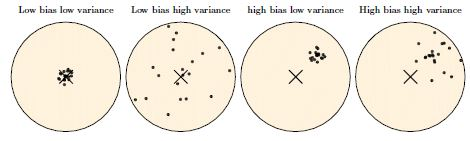
\includegraphics[width=0.9\textwidth]{biasvariance}
  \caption{Bias and variance}\label{fig:biasvariance}
\end{figure}

\begin{figure}[H]
  \centering
  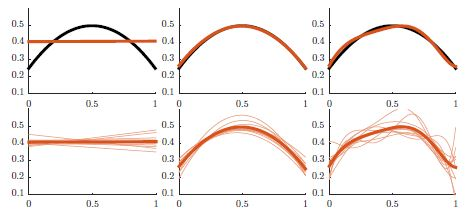
\includegraphics[width=0.9\textwidth]{exampleofbiasvariance}
  \caption{Bias-variance decomposition for the three linear regression models. In the top row is shown the bias term. Namely, how much the average values of the models trained on different random data sets (illustrated with the thick red line) differ from the true mean values of the data illustrated by the black line. In the bottom row is shown the variance term. Namely, how much each model wiggles around the mean of all models.}\label{fig:exampleofbiasvariance}
\end{figure}

%Solve exercise from lecture \cite[p.~49]{lecture1}

From lecture \cite[p.~48]{lecture1} then There are three sources of errors contribute to the EPE (Expected Prediction Error)

\begin{equation}
  \begin{split}
     Err(x_0) =  & \: E[(Y- \hat{f}(x_0))^2 | X = x_0] \\
       =& \: \sigma^2_\varepsilon + [E \hat{f}(x_0) - f(x_0)]^2 + E[\hat{f}(x_0) - E\hat{f}(x_0)]^2 \\
       =& \: \sigma_\varepsilon^2 + \text{Bias}^2 (\hat{f}(x_0)) + \text{Var}(\hat{f}(x_0)) \\
       =& \: \text{Irreducible Error} + \text{Bias}^2 + \text{Variance}
  \end{split}
\end{equation}

Bias Variance trade off and EPE

If a model is not complex enough it produce \textbf{underfit} models, that can't learn the signal from the data.\\

But if a model is too comples, it produce \textbf{overfit} models that memorize the noise instead of the signal

%https://elitedatascience.com/bias-variance-tradeoff

\subsection{Ridge Regression}

Ridge Regression \cite[p.~61]{friedman2016elements} and from \cite[p.~53]{lecture1} then

\begin{itemize}
  \item We wish to lower the variance $\hat{y} = \bm{X} \beta$
  \item Lowering the size of $\beta$ will lower the variance of $\hat{y}$
  \item Lower the size of $\beta$ by shrinkage
  \begin{itemize}
    \item $\hat{\beta}_\text{ridge} = \arg \min\limits_\beta ||y - X \beta ||^2 + \lambda ||\beta||^2$
    \item OLS (Ordinary Linear Squares) criterion plus extra term
    \item $\lambda$ controls the amount of shrinkage
  \end{itemize}
\end{itemize}

and it is Important: Data are centered (mean of each variable is zero) and normalized (variables scaled such that standard deviation equals 1). Centering data removes the mean, causes the shrinkage to shrink
towards zero and Normalizing data puts equal importance to all variables due to the
penalty term $||\beta||^2$

Impose a penalty parameter from \cite[p.~63]{friedman2016elements}

\[
    \hat{\beta}_{\text{ridge}} = \arg \min\limits_{\beta} \left\{\sum_{i=1}^{N} (y_i - \beta_0 - \sum_{j=1}^{P} x_{ij} \beta_j)^2 + \lambda \sum_{j=1}^{P} \beta_j^2\right\}
\]

Where $\lambda \geq 0$ is a complexity parameter that controls that amount of shrinkage.

Writing this to matrix form, we have

\[
    \hat{\beta}_{\text{ridge}} = (\bm{X}^T\bm{X} + \lambda \bm{I})^{-1} \bm{X}^T\bm{y}
\]

where $\bm{I}$ is $p \times p$ identity matrix.

This

\begin{itemize}
  \item Stabilizes the inverse numerically
  \item Ridge regression solutions are available even when $p > n$
\end{itemize}

\section{Linear Classifiers}

\begin{itemize}
  \item Fischer Linear Discriminant Analysis
  \item K-Nearest-Neighbor classification
\end{itemize}

\subsection{Fischer Linear}

Find a linear combination $Z = a^T X$ such that the between-class variance is maximized relative to the within-class variance

\begin{figure}[H]
  \centering
  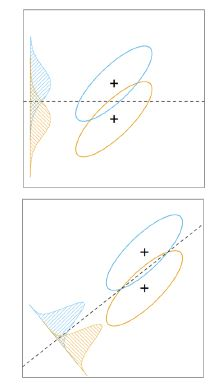
\includegraphics[height=0.5\textwidth]{FLLDA}
  \caption{Example of the Linear Discriminant Analysis}\label{fig:FLLDA}
\end{figure}

Maximize between-class variance $a^T \Sigma_B a$ where

\[
    \Sigma_B = \sum_{j=1}^{K} (\mu_j - \mu)^T(\mu_j - \mu)
\]

Minimize the within-class variance $a^T \Sigma_W a$ where

\[
    \Sigma_W = \sum_{j=1}^{K} \sum_{i=1}^{n_j} (X_{ij} -\mu_j)^T (X_{ij} -\mu_j)
\]

where the group mean is $u_j$ and total mean is $\mu$. Then the separating line is given by

\[
    \max\limits_a \frac{a^T \Sigma_B a}{a^T \Sigma_W a}
\]

from lecture \cite[p.~59]{lecture1}

\section{k-Nearest-Neighbor Classifiers}

Remember to standardize data. If one measurement is 1000 kilometers and a second is 0.01 gram, then the first feature will dominate.

Classify observations according to the majority class of the K nearest neighbors

Small values of $K$  gives low bias, large values will give low variance.

In k-NN classification, the output is a class membership. An object is classified by a majority vote of its neighbors, with the object being assigned to the class most common among its k nearest neighbors (k is a positive integer, typically small). If k = 1, then the object is simply assigned to the class of that single nearest neighbor.

\section{K-Nearest-Neighbors regression}

Estimate the response of an observation as the average response of
the K nearest neighbors.

Define distance measure of proximity, eg Euclidean distance

It is general practice to standardize each variable to mean zero
and variance 1

In k-NN regression, the output is the property value for the object. This value is the average of the values of its k nearest neighbors.

\begin{figure}[H]
  \centering
  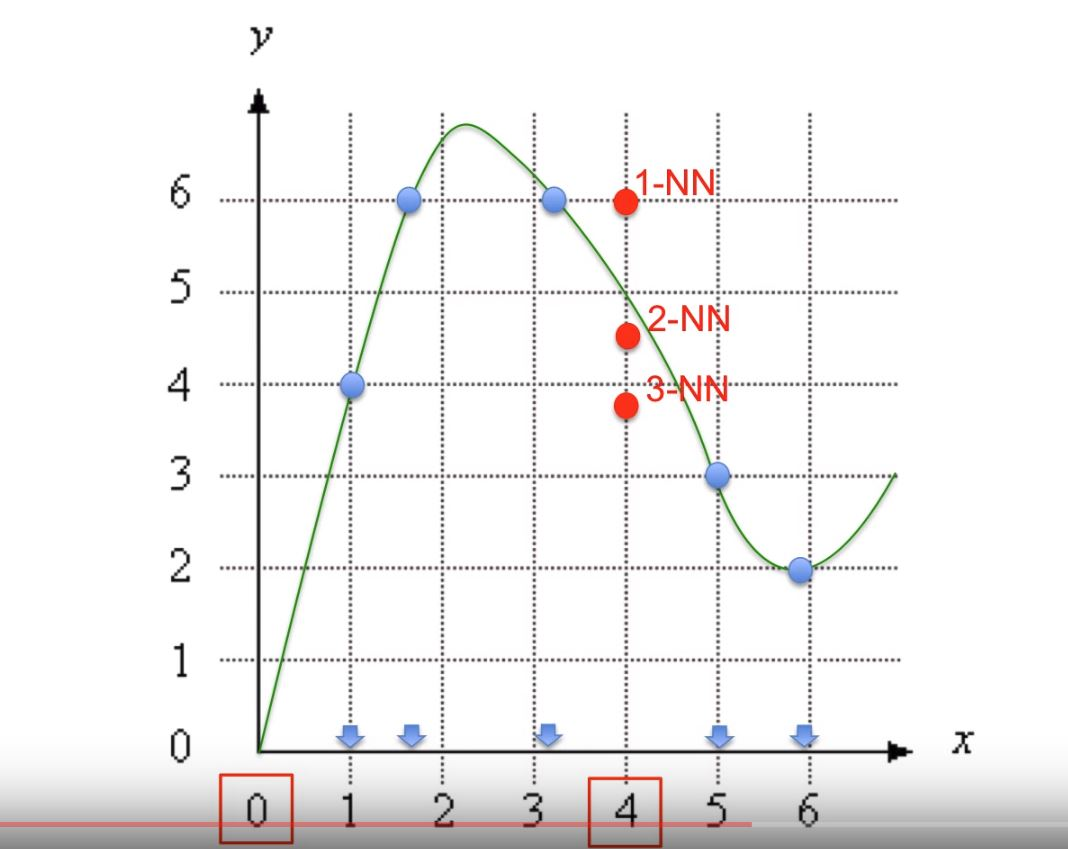
\includegraphics[width=0.9\textwidth]{knnregression}
\end{figure}


